%-----------------------------QUESTÃO------------------------------------
%Cód.: TF3p05q24

\question[\questaopt]Determine o módulo da força de interação entre duas
partículas eletrizadas com \SI{+4,0}{\micro\coulomb} e \SI{-3,0}{\micro\coulomb}, estando elas no vácuo à
distância de \SI{6,0}{\centi \meter} uma da outra.\\
\textbf{Dados}: Constante eletrostática do vácuo $ \cteK $
				
%------------------------------ALTERNATIVAS-----------------------------

		\begin{EnvUplevel}
			\begin{choices}
			
			\choice \SI{10}{\newton}  
			\choice \SI{20}{\newton}
			\correctchoice \SI{30}{\newton}
			\choice \SI{40}{\newton}
			\choice \SI{50}{\newton}
				
			\end{choices}
		\end{EnvUplevel}

%--------------------------SOLUÇÃO---------------------------------------
		
		\begin{EnvUplevel}
		\begin{solution}[2cm]
		{\footnotesize\\
		Como as cargas têm sinais opostos, a interação entre elas é atrativa.
		
		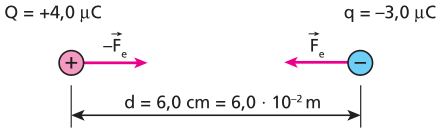
\includegraphics[width=0.4\linewidth]{questoes/imagens/TF3p05q24_1}
	
		Aplicando a Lei de Coulomb a essa interação, temos:
				$$
				\Fel \\
				$$
		Substituindo os valores conhecidos, vem:
				$$
				F_e=\num{9e9}\times\frac{\left| \num{4,0e-6} \times \num{-3,0e-6} \right|}{\left( \num{6,0e-2} \right)^{2}}
				$$
				$$
				F_e=\SI{30}{\newton}
				$$
		}
		
		\end{solution}
		\end{EnvUplevel}
\vspace{\stretch{1}}